\begin{enumerate}[label=\thechapter.\arabic*,ref=\thechapter.\theenumi]
\item A sinusoidal message signal having root mean square value of 4V and frequency of 1 kHz fed to a phase modulator with phase deviation constant 2 rad/volt. If the carrier signal is $c\brak{t} = 2\cos \brak{2\pi 10^6 t}$, the maximum instantaneous frequency of the phase modulated signal (rounded off to one decimal place) is \rule{1cm}{0.05mm} Hz. \hfill(GATE 2021 EC)\\
\solution\\
\iffalse
\documentclass[journal,12pt,twocolumn]{IEEEtran}
\usepackage{amsmath,amssymb,amsfonts,amsthm}
\usepackage{txfonts}
\usepackage{tkz-euclide}
\usepackage[margin=0.25in]{geometry}
\usepackage{pgfplots}
\usepackage{listings}
\usepackage{gvv}
\usepackage[latin1]{inputenc}
\usepackage{adjustbox}
\usepackage{array}
\usepackage{tabularx}
\usepackage{enumitem}
\usepackage{pgf}
\usepackage{lmodern}
\usepackage{circuitikz}
\usepackage{tikz}
\usepackage{graphicx}
\pgfplotsset{width=10cm,compat=1.18}

\begin{document}
\bibliographystyle{IEEEtran}

\vspace{3cm}

\title{}
\author{EE23BTECH11054 -  Sai Krishna Shanigarapu$^{*}$
}
\maketitle
\newpage
\bigskip

\section*{Gate EC 2021}
49. \hspace{2pt} A sinusoidal message signal having root mean square value of 4V and frequency of 1 kHz fed to a phase modulator with phase deviation constant 2 rad/volt. If the carrier signal is $c\brak{t} = 2\cos \brak{2\pi 10^6 t}$, the maximum instantaneous frequency of the phase modulated signal (rounded off to one decimal place) is \rule{1cm}{0.05mm} Hz. \hfill(GATE 2021 EC)\\
\solution\\
\fi
\begin{table}[ht]
    \centering
    \setlength{\arrayrulewidth}{0.3mm}
\setlength{\tabcolsep}{20pt}
\renewcommand{\arraystretch}{1.5}


\begin{tabular}{|c|c|c|}
\hline
Parameter & Description & Value\\
\hline
$f_m$ & Message signal frequency & 1 kHz\\
\hline
$c\brak{t}$ & Carrier signal & $2\cos \brak{2\pi 10^6 t}$\\
\hline
$k_p$ & Phase sensitivity factor & 2 rad $V^{-1}$\\
\hline
$m\brak{t}$ &  message signal & $A_m\sin{2\pi f_m t}$\\
\hline
$f_c$ & Carrier signal frequency & 1 kHz\\
\hline
$A_c$ & Amplitude of carrier signal & 2 \\
\hline
$A_m$ & Amplitude of message signal & \\
\hline
\end{tabular}
    \caption{Input Parameters}
    \label{tab:tab1_gate_2021_ec_49}
\end{table}

\begin{table}[ht]
    \centering
    \setlength{\arrayrulewidth}{0.3mm}
\setlength{\tabcolsep}{20pt}
\renewcommand{\arraystretch}{1.6}


\begin{tabular}{|c|c|c|}
\hline
Parameter & Description & Formula\\
\hline
$m\brak{t}_{rms}$ & rms value of $m\brak{t}$ & $\frac{A_m}{\sqrt{2}}$\\
\hline
$s\brak{t}$ & Phase modulation & $A_c\sin \sbrak{2\pi f_c t + \theta _i\brak{t}}$\\
\hline
$\theta _i\brak{t}$ & phase & $k_p\, m\brak{t}$\\
\hline
\end{tabular}

    \caption{Formulae}
    \label{tab:tab2_gate_2021_ec_49}
\end{table}

Phase Modulation Signal Proof:\\
let $e_m$ and $e_c$ be message and carrier signals, $2\pi f_m$ and $2\pi f_c$ be radial frequencies and $A_m$ and $A_c$ be their amplitudes respectively. Then,
\begin{align}
	e_m &= A_m\cos \brak{2\pi f_m t}\\
	e_c &= A_c \sin \brak{2\pi f_c t} \label{eq:test1_21_ec49}
\end{align}
On rewriting the equation \ref{eq:test1_21_ec49}
\begin{align}
	e &= E_c\sin \brak{\theta}\\
	\theta &= 2\pi f_c t + k_p e_m\\
	&= 2\pi f_c t + k_pE_m\cos \brak{2\pi f_m t}\\
	m_p &= k_p E_m\\
	\theta &= 2\pi f_c t + m_p\cos \brak{2\pi f_m t}\\
	\implies s\brak{t} &= E_c\sin \brak{2\pi f_c t + \underbrace{m_p\cos \brak{2\pi f_m t}}_\text{$\theta_i \brak{t}$}} \label{eq:test2_21_ec49}
\end{align}

\begin{align}
    m\brak{t}_{rms} &= 4V \label{eq:eq1_gate_2021_ec_49} \\
    A_m &= 4\sqrt{2} \label{eq:eq2_gate_2021_ec_49}
\end{align}
From Table \ref{tab:tab1_gate_2021_ec_49}, eq (\ref{eq:eq1_gate_2021_ec_49}) and eq (\ref{eq:eq2_gate_2021_ec_49})
\begin{align}
     m\brak{t} &= 4\sqrt{2}\sin \brak{2 \pi 10^3 t}\\
\end{align}

\begin{figure}[ht]
    \centering
    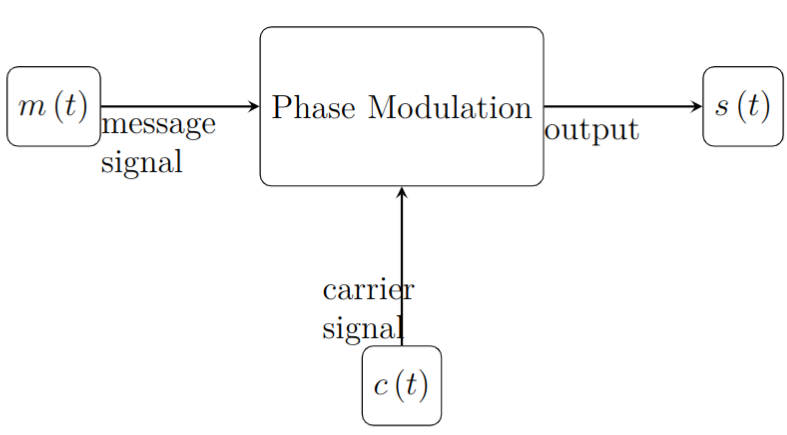
\includegraphics[width=\columnwidth]{2021/EC/49/figs/fig2.png}
    \caption{Block diagram of phase modulation}
    \label{fig:fig1_gate_2021_ec_49}  
\end{figure}
From Table \ref{tab:tab1_gate_2021_ec_49}, \ref{tab:tab2_gate_2021_ec_49} and using eq (\ref{eq:test2_21_ec49}) instantaneous frequency is given as,
\begin{align}
    f_i\brak{t} &= f_c + \frac{1}{2\pi}\, \frac{d}{dt}\theta_i\brak{t}\\
    &= f_c + \frac{1}{2\pi}\, \frac{d}{dt}\sbrak{k_p m\brak{t}}\\
    &= f_c + \frac{1}{2\pi}\, \frac{d}{dt}\brak{4\sqrt{2}\sin \brak{2 \pi 10^3 t}}\\
    &= f_c + \frac{2}{2\pi}\, 4\sqrt{2}\, \brak{2\pi 10^3}\, \brak{\cos \brak{2 \pi 10^3 t}}\\
    &= 1000 + 8\sqrt{2} \text{ x } 10^3 \cos \brak{2\pi 10^3 t}
\end{align}
Thus,
\begin{align}
    \implies f_{i_{max}} &= 1011313.7 \, Hz
\end{align}

\begin{figure}[ht]
    \centering
        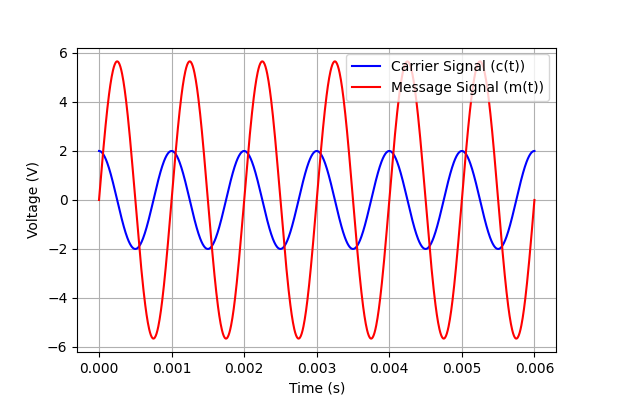
\includegraphics[width=\columnwidth]{2021/EC/49/figs/Figure_1.png}
    \caption{plot of $m\brak{t}$ and $c\brak{t}$}
\end{figure}

%\end{document}

\pagebreak
\item Two discrete-time linear time-invarient systems with impulse responses $h_1[n]=\delta[n-1]+\delta[n+1]$ and $h_2[n]=\delta[n]+\delta[n-1]$ are connected in cascade, where $\delta[n]$ is the Kronecker delta. The impulse response of the cascaded system is   \\
\begin{enumerate}[label=(\alph*)]
    \item $\delta[n-2]+\delta[n+1]$
    \item $\delta[n-1]\delta[n]+\delta[n+1]\delta[n-1]$
    \item $\delta[n-2]+\delta[n-1]+\delta[n]+\delta[n+1]$
    \item $\delta[n]\delta[n-1]+\delta[n-2]\delta[n+1]$
\end{enumerate} \hfill(GATE 2021 EE)\\
\solution
\iffalse
\let\negmedspace\undefined
\let\negthickspace\undefined
\documentclass[journal,12pt,twocolumn]{IEEEtran}
\usepackage{cite}
\usepackage{amsmath,amssymb,amsfonts,amsthm}
\usepackage{algorithmic}
\usepackage{graphicx}
\usepackage{textcomp}
\usepackage{xcolor}
\usepackage{pgfplots}
\usepackage{txfonts}
\usepackage{listings}
\usepackage{enumitem}
\usepackage{mathtools}
\usepackage{gensymb}
\usepackage{comment}
\usepackage[breaklinks=true]{hyperref}
\usepackage{tkz-euclide} 
\usepackage{listings}
\usepackage{gvv}                                        
\def\inputGnumericTable{}                                 
\usepackage[latin1]{inputenc}                                
\usepackage{color}                                            
\usepackage{array}                                            
\usepackage{longtable}                                       
\usepackage{calc}                                             
\usepackage{multirow}                                         
\usepackage{hhline}                                           
\usepackage{ifthen}                                           
\usepackage{lscape}

\newtheorem{theorem}{Theorem}[section]
\newtheorem{problem}{Problem}
\newtheorem{proposition}{Proposition}[section]
\newtheorem{lemma}{Lemma}[section]
\newtheorem{corollary}[theorem]{Corollary}
\newtheorem{example}{Example}[section]
\newtheorem{definition}[problem]{Definition}
\newcommand{\BEQA}{\begin{eqnarray}}
\newcommand{\EEQA}{\end{eqnarray}}
\newcommand{\define}{\stackrel{\triangle}{=}}
\theoremstyle{remark}
\newtheorem{rem}{Remark}
\begin{document}
\parindent 0px
\bibliographystyle{IEEEtran}
\title{GATE: EE - 7.2021}
\author{EE22BTECH11219 - Rada Sai Sujan$^{}$% <-this % stops a space
}
\maketitle
\newpage
\bigskip
\section*{Question}
Two discrete-time linear time-invarient systems with impulse responses $h_1[n]=\delta[n-1]+\delta[n+1]$ and $h_2[n]=\delta[n]+\delta[n-1]$ are connected in cascade, where $\delta[n]$ is the Kronecker delta. The impulse response of the cascaded system is   \\
\begin{enumerate}[label=(\alph*)]
    \item $\delta[n-2]+\delta[n+1]$
    \item $\delta[n-1]\delta[n]+\delta[n+1]\delta[n-1]$
    \item $\delta[n-2]+\delta[n-1]+\delta[n]+\delta[n+1]$
    \item $\delta[n]\delta[n-1]+\delta[n-2]\delta[n+1]$
\end{enumerate} \hfill(GATE 2021 EE)\\
\solution
\fi

\begin{figure}[ht]
    \centering
    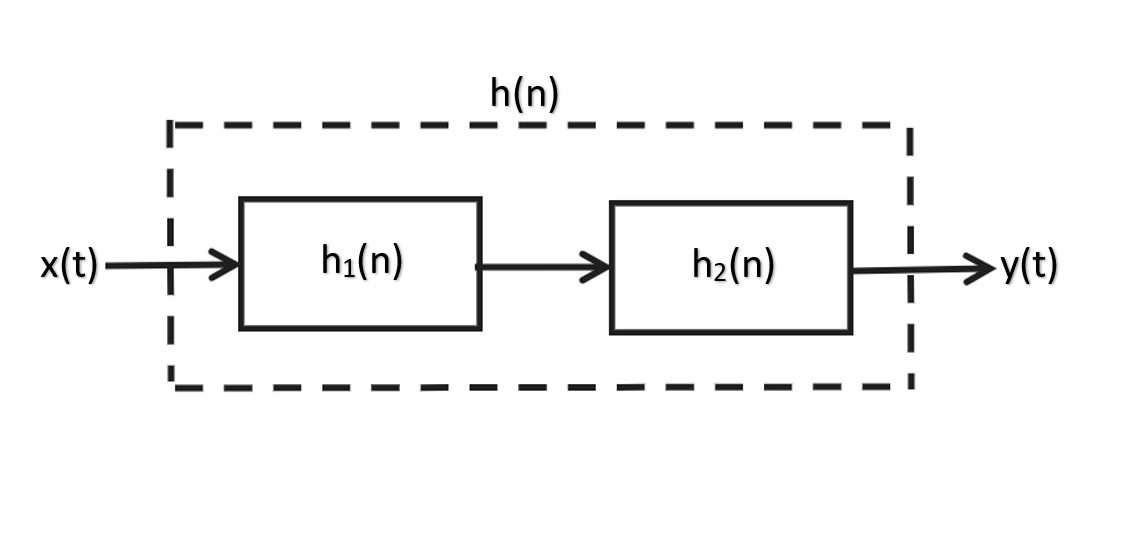
\includegraphics[width=\columnwidth]{2021/EE/7/figs/fig2.png}
    \caption{Block Diagram}
    \label{fig:g2022ee7.2}
\end{figure}  
From the $Z$-transformation pairs,
\begin{align}
    \delta[n] &\overset{\mathcal{Z}}{ \longleftrightarrow} 1  \label{eqn:g22ee7.1}  \\
    x\brak{n-k} &\overset{\mathcal{Z}}{ \longleftrightarrow} z^{-k}X\brak{z} \label{eqn:g22ee7.2}   \\
    x_1\brak{n}\ast x_2\brak{n} &\overset{\mathcal{Z}}{ \longleftrightarrow} X_1\brak{z}X_2\brak{z} \label{eqn:g22ee7.3}
\end{align}
If $h_1\brak{n}$ and $h_2\brak{n}$ are cascade connected then the resultant impulse can be given by:
\begin{align}
    h\brak{n}&=h_1\brak{n}\ast h_2\brak{n}    \\
    \implies H\brak{z}&=H_1\brak{z}H_2\brak{z}    \\
    H\brak{z}&=\brak{z^{-1}+z}\brak{1+z^{-1}}   \\
    &=\brak{z^{-1}+z^{-2}+z+1}, \quad \abs{z}\neq 0
\end{align}
Using the $Z$-transformation pairs to find the the inverse $Z$-transform,
\begin{align}
    h\brak{n}&=\delta[n-2]+\delta[n-1]+\delta[n]+\delta[n+1]
\end{align}
\begin{figure}[ht]
    \centering
    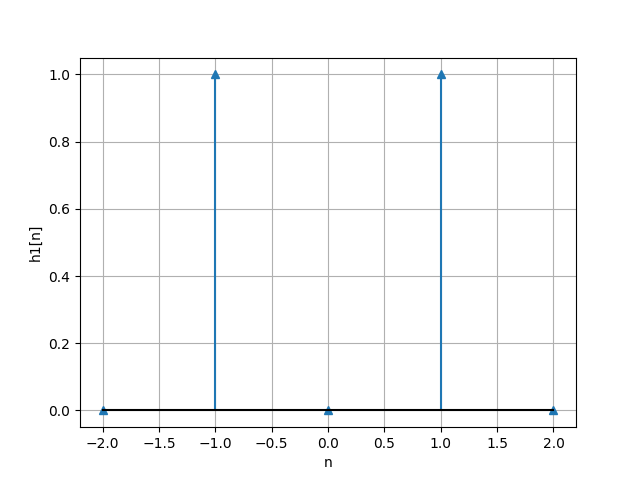
\includegraphics[width=\columnwidth]{2021/EE/7/figs/fig3.png}
    \caption{$h_1\brak{n}$ $vs$ $n$ graph}
    \label{fig:g2022ee7.3}
\end{figure}     
\begin{figure}[ht]
    \centering
    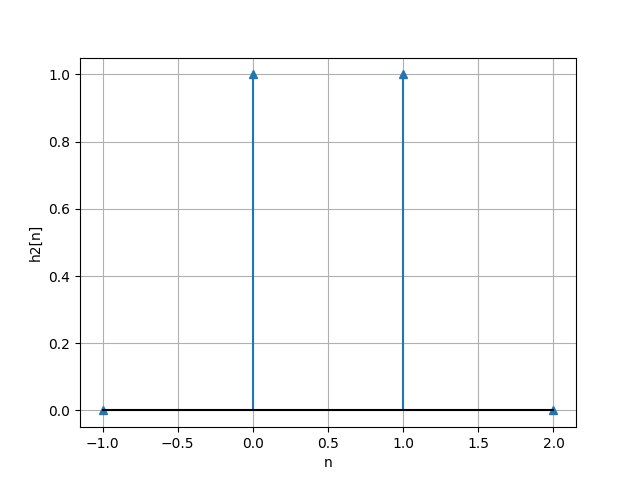
\includegraphics[width=\columnwidth]{2021/EE/7/figs/fig4.png}
    \caption{$h_2\brak{n}$ $vs$ $n$ graph}
    \label{fig:g2022ee7.4}
\end{figure}     
\begin{figure}[ht]
    \centering
    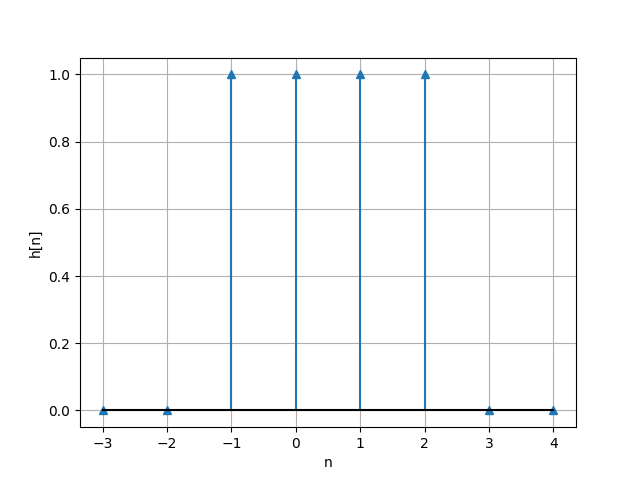
\includegraphics[width=\columnwidth]{2021/EE/7/figs/fig1.png}
    \caption{$h\brak{n}$ $vs$ $n$ graph}
    \label{fig:g2022ee7.1}
\end{figure}

\pagebreak
\item Consider a superheterodyne receiver tuned to 600 kHz. If the local oscillator feeds a 1000 kHz signal to the mixer, the image frequency (in integer) is \underline{\hspace{1cm}} kHz.
\hfill(GATE EC 2021)\\
\solution
\iffalse
\documentclass{article}
\usepackage{tikz}
\usetikzlibrary{positioning, arrows.meta, shapes.geometric, shapes.multipart}
\usepackage{amsmath}

\begin{document}

Consider a superheterodyne receiver tuned to 600 kHz. If the local oscillator feeds a 1000 kHz signal to the mixer, the image frequency (in integer) is \underline{\hspace{1cm}} kHz.
\hfill(GATE EC 2021)\\

\textbf{Solution:}
\fi
\begin{table}[h]
    \centering
    \begin{tabular}{|c|c|c|}
        \hline
        \textbf{Parameter} & \textbf{Symbol} & \textbf{Value} \\
        \hline
        Receiver Frequency & \(f_r\) & 600 kHz \\
        \hline
        Local Oscillator Frequency & \(f_l\) & 1000 kHz \\
        \hline
        Image Frequency & \(f_i\) & \underline{\hspace{2cm}} kHz \\
        \hline
    \end{tabular}
    \caption{Given Parameters with Symbols}
\end{table}

Let \(f_x\) be the intermediate frequency given by \(|f_l - f_r|\).
\begin{align}
    f_x &= |1000-600| = 400 \, \text{kHz}
\end{align}
\begin{figure}[htb]
 \centering
\begin{tikzpicture}
    \draw (0,0) -- (6,0);
    \draw[thick,->] (1,0) -- node[below=4mm] {$f_r$} (1,1);
    \draw[thick,->] (3,0) -- node[below=14mm] {$f_l$} (3,3);
    \draw[thick,->] (5,0) --  node[below=4mm] {$f_i$}(5,1);
    \draw[<->] (1.25,0.5) --node[above] {$f_x$}(2.75,0.5);
    \draw[<->] (3.25,0.5) --node[above] {$f_x$}(4.75,0.5);
\end{tikzpicture}
 \caption{Diagram}
    \label{fig:reflection}
\end{figure}



From the above diagram, we can observe that:
\begin{align}
    f_i &= f_r+2(f_x) = 600+2(400)=1400 \, \text{kHz}
\end{align}
Therefore the Image frequency is \textbf{1400 kHz}
\begin{figure}
    \centering
    \begin{tikzpicture}[
        block/.style={draw, rectangle, minimum height=1.5cm, text width=3cm, align=center},
        arrow/.style={->, >=Stealth},
        node distance=2cm
    ]

    % Nodes
    \node[block] (mixer) {Mixer};
    \node[block, below=of mixer] (if) {Intermediate\\Frequency\\($f_x = 400$ kHz)};
    \node[block, below=of if] (lo) {Local Oscillator\\($f_r = 1000$ kHz)};
    \node[block, below=of lo] (rf) {RF Signal\\($f_l = 600$ kHz)};
    \node[block, right=of if, xshift=2cm] (image) {Image Frequency\\($f_i = 1400$ kHz)};

    % Arrows
    \draw[arrow] (rf) -- (lo);
    \draw[arrow] (lo) -- (if);
    \draw[arrow] (mixer) -- (if);
    \draw[arrow] (if) -- (image);

    \end{tikzpicture}
    \caption{Superheterodyne Receiver Block Diagram}
\end{figure}


%\end{document}


\pagebreak
\item Consider a unity feedback system with closed loop transfer function
\begin{align*}
\frac{C\brak{s}}{R\brak{s}} &= \frac{s + 90}{s^2 + 10s + 90}
\end{align*}
The steady state error with respect to a unit ramp input is \rule{1cm}{0.15mm} .
\hfill(GATE 2021 BM) \\
\solution
\iffalse
\let\negmedspace\undefined
\let\negthickspace\undefined
\documentclass[journal,12pt,twocolumn]{IEEEtran}
\usepackage{cite}
\usepackage{amsmath,amssymb,amsfonts,amsthm}
\usepackage{algorithmic}
\usepackage{graphicx}
\usepackage{textcomp}
\usepackage{xcolor}
\usepackage{txfonts}
\usepackage{listings}
\usepackage{enumitem}
\usepackage{mathtools}
\usepackage{gensymb}
\usepackage{comment}
\usepackage[breaklinks=true]{hyperref}
\usepackage{tkz-euclide}
\usepackage{listings}
\usepackage{gvv}
\def\inputGnumericTable{}
\usepackage[latin1]{inputenc}
\usepackage{color}
\usepackage{array}
\usepackage{longtable}
\usepackage{calc}
\usepackage{multirow}
\usepackage{hhline}
\usepackage{ifthen}
\usepackage{lscape}

\newtheorem{theorem}{Theorem}[section]
\newtheorem{problem}{Problem}
\newtheorem{proposition}{Proposition}[section]
\newtheorem{lemma}{Lemma}[section]
\newtheorem{corollary}[theorem]{Corollary}
\newtheorem{example}{Example}[section]
\newtheorem{definition}[problem]{Definition}
\newcommand{\BEQA}{\begin{eqnarray}}
\newcommand{\EEQA}{\end{eqnarray}}
\newcommand{\define}{\stackrel{\triangle}{=}}
\theoremstyle{remark}
\newtheorem{rem}{Remark}
\begin{document}

\bibliographystyle{IEEEtran}
\vspace{3cm}

\title{GATE 2021 BM 46}
\author{EE23BTECH11007 - Aneesh Kadiyala$^{*}$% <-this % stops a space
}
\maketitle
\newpage
\bigskip

\renewcommand{\thefigure}{\theenumi}
\renewcommand{\thetable}{\theenumi}

\vspace{3cm}
\textbf{Question:} Consider a unity feedback system with closed loop transfer function
\begin{align*}
\frac{C\brak{s}}{R\brak{s}} &= \frac{s + 90}{s^2 + 10s + 90}
\end{align*}
The steady state error with respect to a unit ramp input is \rule{1cm}{0.15mm} . \brak{\text{rounded off to one decimal}}

\hfill(GATE 2021 BM)
\\
\solution
\\
\fi
\begin{figure}[h!]
\centering
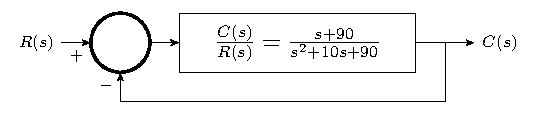
\includegraphics[width=\columnwidth]{2021/BM/46/figs/block-diagram.pdf}
\caption{Block Diagram of the System}
\label{fig:2021bm46-1}
\end{figure}

\begin{align}
\frac{C\brak{s}}{R\brak{s}} &= \frac{s + 90}{s^2 + 10s + 90}
\end{align}
where $C\brak{s}$ is the output and $R\brak{s}$ is the input.
Given that input is unit ramp function:
\begin{align}
r\brak{t} &= tu\brak{t} \\
\implies R\brak{s} &= \frac{1}{s^2} \\
\implies C\brak{s} &= \frac{s + 90}{s^2\brak{s^2+10s+90}} \\
E\brak{s} &= R\brak{s} - C\brak{s} \\
&= \frac{s^2+9s}{s^2\brak{s^2+10s+90}}
\end{align}
Steady state error is:
\begin{align}
\lim_{s\to0}{sE\brak{s}} &= \frac{s + 9}{s^2 + 10s + 90} \\
&= \frac{1}{10}
\end{align}
$\therefore$ steady state error for unit ramp input is 0.1.
\begin{figure}[h!]
\centering
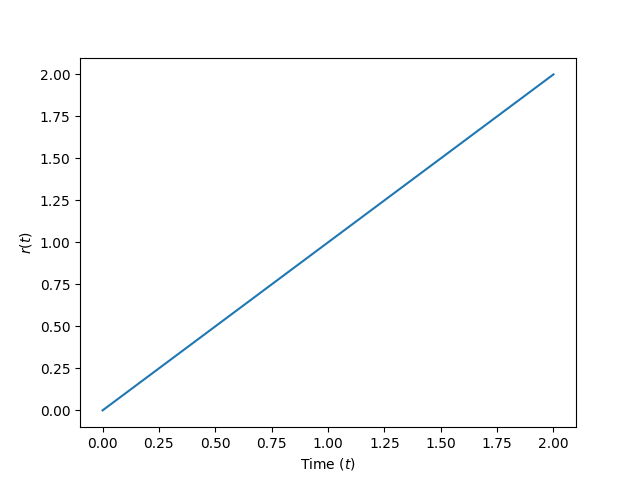
\includegraphics[width=\columnwidth]{2021/BM/46/figs/r_t.png}
\caption{Plot of $r\brak{t}$ vs $t$}
\label{fig:2021bm46-2}
\end{figure}
\begin{align}
C\brak{s} &= \frac{s + 90}{s^2\brak{s^2+10s+90}} \\
&= -\frac{1}{10s} + \frac{1}{s^2} + \frac{s}{10\brak{s^2 + 10s + 90}} \\
&= -\frac{1}{10s} + \frac{1}{s^2} + \frac{s + 5}{\brak{s+5}^2+65} - \frac{1}{2}\brak{\frac{1}{\brak{s+5}^2+65}}
\end{align}
\begin{align}
c\brak{t} &= u\brak{t}\brak{-\frac{1}{10} + t + \frac{e^{-5t}}{10} \cos{\brak{\sqrt{65}t}} - \frac{e^{-5t}}{2\sqrt{65}}\sin{\brak{\sqrt{65}t}}}
\end{align}
\begin{figure}[h!]
\centering
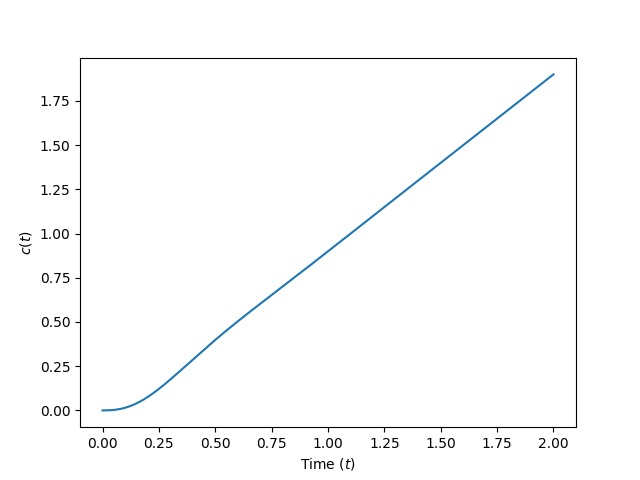
\includegraphics[width=\columnwidth]{2021/BM/46/figs/c_t.png}
\caption{Plot of $c\brak{t}$ vs $t$}
\label{fig:2021bm46-3}
\end{figure}
\begin{align}
E\brak{s} &= R\brak{s} - C\brak{s} \\
\implies e\brak{t} &= r\brak{t} - c\brak{t} \\
&= u\brak{t}\brak{\frac{1}{10} - \frac{e^{-5t}}{10} \cos{\brak{\sqrt{65}t}} + \frac{e^{-5t}}{2\sqrt{65}}\sin{\brak{\sqrt{65}t}}}
\end{align}
\begin{figure}[h!]
\centering
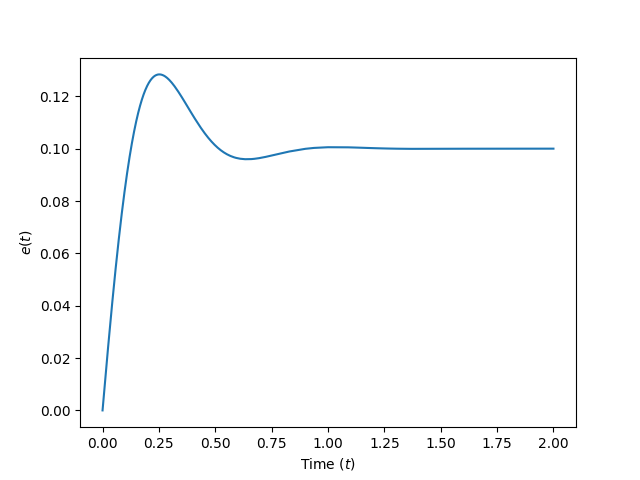
\includegraphics[width=\columnwidth]{2021/BM/46/figs/e_t.png}
\caption{Plot of $e\brak{t}$ vs $t$}
\label{fig:2021bm46-4}
\end{figure}
\begin{align}
\text{Feedback Gain } &= \frac{\frac{C\brak{s}}{R\brak{s}}}{1 + \frac{C\brak{s}}{R\brak{s}}} \\
&= \frac{s + 90}{s^2 + 11s + 180}
\end{align}
\item A unit step input is applied to a system with impulse response H\brak{s} = $\frac{1- \frac{s}{\omega{_z}}}{1+\frac{s}{\omega{_p}}}$ at t=0. The output of the system $y\brak{t}$ at t=$0^+$ is:
\begin{enumerate}[label=\alph*)]
 \item 1
 \item $-\frac{\omega{_z}}{\omega{_p}}$
 \item $-\frac{\omega{_p}}{\omega{_z}}$
 \item 0
\end{enumerate} \hfill(GATE 2021 BM)\\
\solution
\iffalse
\let\negmedspace\undefined
\let\negthickspace\undefined
\documentclass[journal,12pt,onecolumn]{IEEEtran}
\usepackage{cite}
\usepackage{amsmath,amssymb,amsfonts,amsthm}
\usepackage{algorithmic}
\usepackage{graphicx}
\usepackage{textcomp}
\usepackage{xcolor}
\usepackage{txfonts}
\usepackage{listings}
\usepackage{enumitem}
\usepackage{mathtools}
\usepackage{gensymb}
\usepackage{circuitikz}
\usepackage{tkz-euclide} % loads  TikZ and tkz-base
\usepackage{listings}
\usetikzlibrary{positioning,arrows,shapes}


\newtheorem{theorem}{Theorem}[section]
\newtheorem{problem}{Problem}
\newtheorem{proposition}{Proposition}[section]
\newtheorem{lemma}{Lemma}[section]
\newtheorem{corollary}[theorem]{Corollary}
\newtheorem{example}{Example}[section]
\newtheorem{definition}[problem]{Definition}
%\newtheorem{thm}{Theorem}[section] 
%\newtheorem{defn}[thm]{Definition}
%\newtheorem{algorithm}{Algorithm}[section]
%\newtheorem{cor}{Corollary}
\newcommand{\BEQA}{\begin{eqnarray}}
\newcommand{\EEQA}{\end{eqnarray}}
\newcommand{\system}[1]{\stackrel{#1}{\rightarrow}}

\newcommand{\define}{\stackrel{\triangle}{=}}
\theoremstyle{remark}
\newtheorem{rem}{Remark}
%\bibliographystyle{ieeetr}
\begin{document}
%
\providecommand{\pr}[1]{\ensuremath{\Pr\left(#1\right)}}
\providecommand{\prt}[2]{\ensuremath{p_{#1}^{\left(#2\right)} }}        % own macro for this question
\providecommand{\qfunc}[1]{\ensuremath{Q\left(#1\right)}}
\providecommand{\sbrak}[1]{\ensuremath{{}\left[#1\right]}}
\providecommand{\lsbrak}[1]{\ensuremath{{}\left[#1\right.}}
\providecommand{\rsbrak}[1]{\ensuremath{{}\left.#1\right]}}
\providecommand{\brak}[1]{\ensuremath{\left(#1\right)}}
\providecommand{\lbrak}[1]{\ensuremath{\left(#1\right.}}
\providecommand{\rbrak}[1]{\ensuremath{\left.#1\right)}}
\providecommand{\cbrak}[1]{\ensuremath{\left\{#1\right\}}}
\providecommand{\lcbrak}[1]{\ensuremath{\left\{#1\right.}}
\providecommand{\rcbrak}[1]{\ensuremath{\left.#1\right\}}}
\newcommand{\sgn}{\mathop{\mathrm{sgn}}}
\providecommand{\abs}[1]{\left\vert#1\right\vert}
\providecommand{\res}[1]{\Res\displaylimits_{#1}} 
\providecommand{\norm}[1]{\left\lVert#1\right\rVert}
%\providecommand{\norm}[1]{\lVert#1\rVert}
\providecommand{\mtx}[1]{\mathbf{#1}}
\providecommand{\mean}[1]{E\left[ #1 \right]}
\providecommand{\cond}[2]{#1\middle|#2}
\providecommand{\fourier}{\overset{\mathcal{F}}{ \rightleftharpoons}}
\newenvironment{amatrix}[1]{%
  \left(\begin{array}{@{}*{#1}{c}|c@{}}
}{%
  \end{array}\right)
}
\providecommand{\hilbert}{\overset{\mathcal{H}}{ \rightleftharpoons}}
\providecommand{\system}{\overset{\mathcal{H}}{ \longleftrightarrow}}
	%\newcommand{\solution}[2]{\textbf{Solution:}{#1}}
\newcommand{\solution}{\noindent \textbf{Solution: }}
\newcommand{\cosec}{\,\text{cosec}\,}
\providecommand{\dec}[2]{\ensuremath{\overset{#1}{\underset{#2}{\gtrless}}}}
\newcommand{\myvec}[1]{\ensuremath{\begin{pmatrix}#1\end{pmatrix}}}
\newcommand{\mydet}[1]{\ensuremath{\begin{vmatrix}#1\end{vmatrix}}}
\newcommand{\myaugvec}[2]{\ensuremath{\begin{amatrix}{#1}#2\end{amatrix}}}
\providecommand{\rank}{\text{rank}}
\providecommand{\pr}[1]{\ensuremath{\Pr\left(#1\right)}}
\providecommand{\qfunc}[1]{\ensuremath{Q\left(#1\right)}}
	\newcommand*{\permcomb}[4][0mu]{{{}^{#3}\mkern#1#2_{#4}}}
\newcommand*{\perm}[1][-3mu]{\permcomb[#1]{P}}
\newcommand*{\comb}[1][-1mu]{\permcomb[#1]{C}}
\providecommand{\qfunc}[1]{\ensuremath{Q\left(#1\right)}}
\providecommand{\gauss}[2]{\mathcal{N}\ensuremath{\left(#1,#2\right)}}
\providecommand{\diff}[2]{\ensuremath{\frac{d{#1}}{d{#2}}}}
\providecommand{\myceil}[1]{\left \lceil #1 \right \rceil }
\newcommand\figref{Fig.~\ref}
\newcommand\tabref{Table~\ref}
\newcommand{\sinc}{\,\text{sinc}\,}
\newcommand{\rect}{\,\text{rect}\,}
%%
%	%\newcommand{\solution}[2]{\textbf{Solution:}{#1}}
%\newcommand{\solution}{\noindent \textbf{Solution: }}
%\newcommand{\cosec}{\,\text{cosec}\,}
%\numberwithin{equation}{section}
%\numberwithin{equation}{subsection}
%\numberwithin{problem}{section}
%\numberwithin{definition}{section}
%\makeatletter
%\@addtoreset{figure}{problem}
%\makeatother

%\let\StandardTheFigure\thefigure
\let\vec\mathbf

\bibliographystyle{IEEEtran}





\bigskip

\renewcommand{\thefigure}{\theenumi}
\renewcommand{\thetable}{\theenumi}
%\renewcommand{\theequation}{\theenumi}


\title{GATE 2021 BM}
\author{Praful Kesavadas\\ EE23BTECH11049}
\maketitle

\textbf{Q:27}A unit step input is applied to a system with impulse response H\brak{s} = $\frac{1- \frac{s}{\omega{_z}}}{1+\frac{s}{\omega{_p}}}$ at t=0. The output of the system $y\brak{t}$ at t=$0^+$ is:
\begin{enumerate}[label=\alph*)]
 \item 1
 \item $-\frac{\omega{_z}}{\omega{_p}}$
 \item $-\frac{\omega{_p}}{\omega{_z}}$
 \item 0
\end{enumerate}
\solution\\
\fi
Given, input signal $$x\brak{t}= u\brak{t}$$
\begin{align}
 Y\brak{s} &= H\brak{s}.X\brak{s}\\
 &= \frac{1}{s}.\frac{1- \frac{s}{\omega{_z}}}{1+\frac{s}{\omega{_p}}}
\end{align}
By initial value theorem, 
\begin{align}
 y\brak{t=0^+} &= \lim_{s\to\infty} sY\brak{s}\\
 &= \lim_{s\to\infty} \frac{1- \frac{s}{\omega{_z}}}{1+\frac{s}{\omega{_p}}}\\
 &= \lim_{s\to\infty} \frac{\frac{1}{s}- \frac{1}{\omega{_z}}}{\frac{1}{s}+\frac{1}{\omega{_p}}}\\
 &= -\frac{\omega{_p}}{\omega{_z}}
\end{align}
Hence, option \brak{c} is correct
%\end{document}


\item In the block diagram shown below, an infinite tap FIR filter with transfer function $H\brak{z}=\frac{Y\brak{z}}{X\brak{z}}$ is realized. If $H\brak{z}=\frac{1}{1-0.5z^{-1}}$.\\the value of $\alpha$ is
\begin{figure}[h]
    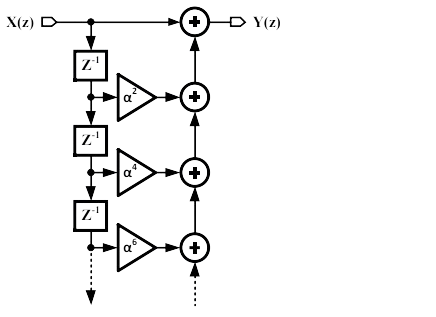
\includegraphics[width=1\columnwidth]{2021/BM/31/figs/questionfig.png}
    \label{fig:question31bm}
\end{figure} \hfill(GATE 2021 BM)\\
\solution
 \iffalse
\let\negmedspace\undefined
\let\negthickspace\undefined
\documentclass[journal,12pt,twocolumn]{IEEEtran}
\usepackage{cite}
\usepackage{amsmath,amssymb,amsfonts,amsthm}
\usepackage{algorithmic}
\usepackage{graphicx}
\usepackage{textcomp}
\usepackage{xcolor}
\usepackage{txfonts}
\usepackage{listings}
\usepackage{enumitem}
\usepackage{mathtools}
\usepackage{gensymb}
\usepackage{comment}
\usepackage{tikz}
\usepackage[breaklinks=true,hidelinks]{hyperref}
\usepackage{tkz-euclide} 
\usepackage{listings}
\usepackage{gvv}
\def\inputGnumericTable{}
\usepackage[latin1]{inputenc}                              
\usepackage{color} 
\usepackage{array}                                            
\usepackage{longtable}                                       
\usepackage{calc}                                             
\usepackage{multirow}                                         
\usepackage{hhline}                                           
\usepackage{ifthen}                                           
\usepackage{lscape}

\newtheorem{theorem}{Theorem}[section]
\newtheorem{problem}{Problem}
\newtheorem{proposition}{Proposition}[section]
\newtheorem{lemma}{Lemma}[section]
\newtheorem{corollary}[theorem]{Corollary}
\newtheorem{example}{Example}[section]
\newtheorem{definition}[problem]{Definition}
\newcommand{\BEQA}{\begin{eqnarray}}
\newcommand{\EEQA}{\end{eqnarray}}
\newcommand{\define}{\stackrel{\triangle}{=}}
\theoremstyle{remark}
\newtheorem{rem}{Remark}
\begin{document}

\bibliographystyle{IEEEtran}
\vspace{3cm}

\title{GATE 2021 BM Q-31}
\author{EE23BTECH11207 -KAILASH.C$^{*}$% <-this % stops a space
}
\maketitle
\newpage
\bigskip

\renewcommand{\thefigure}{\theenumi}
\renewcommand{\thetable}{\theenumi}
In the block diagram shown below, an infinite tap FIR filter with transfer function $H\brak{z}=\frac{Y\brak{z}}{X\brak{z}}$ is realized. If $H\brak{z}=\frac{1}{1-0.5z^{-1}}$.\\the value of $\alpha$ is
\begin{figure}[h]
    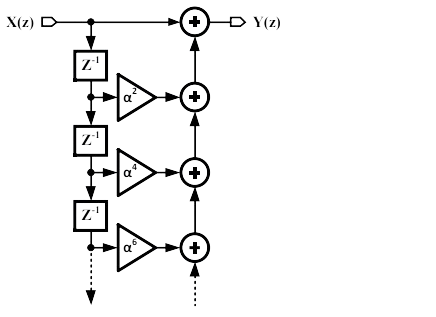
\includegraphics[width=1\columnwidth]{2021/BM/31/figs/questionfig.png}
    \label{fig:question31bm}
\end{figure} \hfill(GATE 2021 BM)\\
\solution
\fi
\begin{table}[h]
\begin{tabular}{|l|l|l|}
\hline
\textbf{Parameter} & \textbf{Definition}\\ \hline
$H\brak{z} & $\frac{1}{1-0.5z^{-1}}$ \\ \hline
\end{tabular}
\caption{Parameter Table}
\label{tab:gate.bm.31.2021}
\end{table}
\\
From diagram we have:
\begin{align}
    Y\brak{z}&=X\brak{z}\brak{\sum_{n=0}^{\infty}\brak{z^{-1}\alpha^{2}}^n}\label{eq:311_bm}
\end{align}
Dividing by $X\brak{z}$ in both sides:
\begin{align}
    \frac{Y\brak{z}}{X\brak{z}}&=\sum_{n=0}^{\infty}\brak{z^{-1}\alpha^{2}}^n\label{eq:312_bm}\\
    \implies H\brak{z}&=\sum_{n=0}^{\infty}\brak{z^{-1}\alpha^{2}}^n\label{eq:313_bm}\\
    \frac{1}{1-0.5z^{-1}}&=\sum_{n=0}^{\infty}\brak{z^{-1}\alpha^{2}}^n\label{eq:314_bm}\\
\frac{1}{1-0.5z^{-1}}&=\frac{1}{1-z^{-1}\alpha^{2}}\label{eq:315_bm}\\
\implies \alpha&=\frac{1}{\sqrt{2}}\label{eq:316_bm}
\end{align}

\pagebreak
\item A unity feedback system that uses proportional-integral (PI) control is shown in the figure.
 \begin{figure}[!ht]    
    \centering
\graphicspath{ {2021/EC/48/figs} }
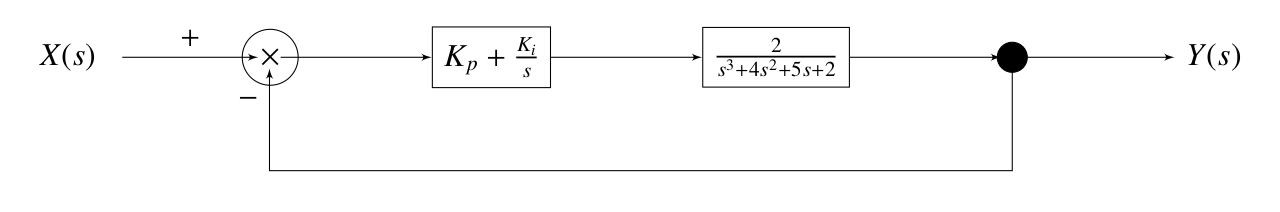
\includegraphics[width=\columnwidth]{figure_1}
\label{figure:ee25-gate4-graph}
\end{figure}
The stability of the overall system is controlled by tuning the PI control parameters $K_p$ and $K_i$. The maximum value of $K_i$ that can be chosen so as to keep the overall system stable or, in the worst case, marginally stable (\textit{rounded off to three decimal places}) is?
\hfill{(GATE EC 2021)}\\
\solution
\iffalse
\let\negmedspace\undefined
\let\negthickspace\undefined
\documentclass[journal,12pt,onecolumn]{IEEEtran}
\usepackage{cite}
\usepackage{amsmath,amssymb,amsfonts,amsthm}
\usepackage{algorithmic}
\usepackage{graphicx}
\usepackage{textcomp}
\usepackage{xcolor}
\usepackage{txfonts}
\usepackage{listings}
\usepackage{enumitem}
\usepackage{circuitikz}
\usepackage{mathtools}
\usepackage{gensymb}
\usepackage{comment}
\usepackage[breaklinks=true]{hyperref}
\usepackage{tkz-euclide} 
\usepackage{listings}
\usepackage{gvv}    
\usepackage{enumitem}
\usepackage{amsmath}
\def\inputGnumericTable{}                                 
\usepackage[latin1]{inputenc}                                
\usepackage{color}                                            
\usepackage{array}                                            
\usepackage{longtable}                                       
\usepackage{calc}                                             
\usepackage{multirow}                                         
\usepackage{hhline}                                           
\usepackage{ifthen}                                           
\usepackage{lscape}
\usepackage{tabularx}
\usepackage[italicdiff]{physics}
\usepackage{mathrsfs}
\usetikzlibrary{arrows,positioning}


\newtheorem{theorem}{Theorem}[section]
\newtheorem{problem}{Problem}
\newtheorem{proposition}{Proposition}[section]
\newtheorem{lemma}{Lemma}[section]
\newtheorem{corollary}[theorem]{Corollary}
\newtheorem{example}{Example}[section]
\newtheorem{definition}[problem]{Definition}
\newcommand{\BEQA}{\begin{eqnarray}}
\newcommand{\EEQA}{\end{eqnarray}}
\newcommand{\define}{\stackrel{\triangle}{=}}
\theoremstyle{remark}
\newtheorem{rem}{Remark}
\begin{document}
\bibliographystyle{IEEEtran}
\vspace{3cm}

\title{GATE:2021 - EC 48 }
\author{EE23BTECH11025 - Anantha Krishnan $^{}$% <-this % stops a space
}
\maketitle
\bigskip



\section{question}
A unity feedback system that uses proportional-integral (PI) control is shown in the figure.
 \begin{figure}[!ht]    
    \centering
\graphicspath{ {2021/EC/48/figs} }
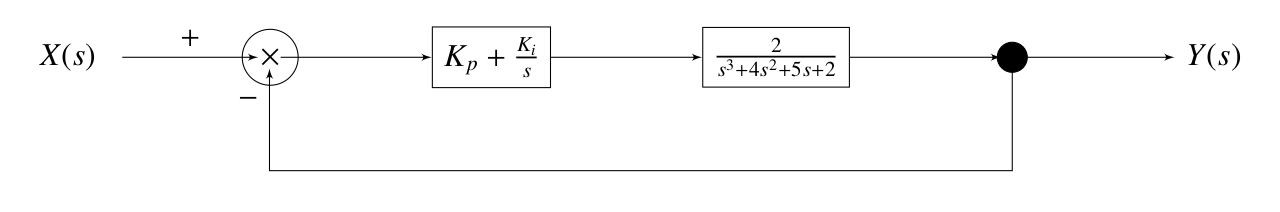
\includegraphics[width=\columnwidth]{figure_1}
\label{figure:ee25-gate4-graph}
\end{figure}
The stability of the overall system is controlled by tuning the PI control parameters $K_p$ and $K_i$. The maximum value of $K_i$ that can be chosen so as to keep the overall system stable or, in the worst case, marginally stable (\textit{rounded off to three decimal places}) is?
\hfill{(GATE EC 2021)}\\
 



\textbf{Solutions :}
\fi
    
\begin{table}[ht!]
\centering
\begin{tabular}{ |c|c|c| } 
 \hline
Symbols & Description & Values  \\
\hline
$P(s)$ & Plant transfer function & $\frac{2}{s^3+4s^2+5s+2}$ \\
 \hline
 $C(s)$ & PI controller transfer function &$K_p+\frac{K_i}{s}$\\
 \hline
$G(s)$ & Closed loop transfer function &$\frac{P(s)C(s)}{1+P(s)C(s)}$\\
 \hline
$Z$ & Number of zeroes with positive real part in $1+P(s)C(s)$ &?\\
 \hline
 $N$ & Total number of anticlockwise encirclements about $-1+0j$ in Nyquist plot & ?\\
\hline
$P$ & Number of poles with positive real part in $P(s)C(s)$ &?\\
\hline
\end{tabular}
\caption{Parameters, Descriptions, and Values}
\label{table:ee25-ec48-gate2021}
\end{table}




    From table \ref{table:ee25-ec48-gate2021}, the characteristic equation is given as:
    \begin{align}
        1+\brak{K_p+\frac{K_i}{s}}\brak{\frac{2}{s^3+4s^2+5s+2}} &= 0\\
        s^4+4s^3+5s^2+(2+2K_p)s+2K_i &=0 \label{eq:gate 2021 eq:4}
    \end{align}
    For the system to be stable, there must be no sign changes in the first column of the routh array for the above equation. From $\eqref{eq:gate 2021 eq:4}$
    \begin{align}
    \begin{array}{c|cccc}
        s^4 & 1 & 5 & 2K_i \\
        s^3 & 4 & (2 + 2K_p) & 0 \\
        s^2 & \frac{18-2K_p}{4} & 2K_i & 0 \\
        s^1 &  \frac{\brak{\frac{18-2K_p}{4}}\brak{2 + 2K_p}-8K_i}{\frac{18-2K_p}{4}} & 0 & 0\\
        s^0 & 2K_i &0 &0 \\
        \end{array}\\
        \end{align}
        \begin{align}
            \frac{18-2K_p}{4} &> 0\\
            \implies K_p &< 9 \label{eq:gate 2021 eq:1}\\
            \frac{\brak{\frac{18-2K_p}{4}}\brak{2 + 2K_p}-8K_i}{\frac{18-2K_p}{4}} &> 0\label{eq:gate 2021 eq:2}\\
        K_i &>0 \label{eq:gate 2021 eq:3}
    \end{align}
    For marginal stability, assuming 3 cases while maximising $K_i$ and checking if the above inequalities hold.
    \begin{enumerate}
        \item $K_p=9$\\
         \begin{align}
       \brak{\lim_{K_p\to9^-} \frac{\brak{\frac{18-2K_p}{4}}\brak{2 + 2K_p}-8K_i}{\frac{18-2K_p}{4}} > 0} &\cap \brak {K_i > 0}\\
       \brak{\lim_{K_p\to9^-} -8K_i > 0} &\cap \brak{{K_i > 0}}\\
  \implies K_p=9 , \forall K_i &\epsilon (\phi)
    \end{align}
    \item  $K_i=0$\\
    \begin{align}
        \brak{\brak{\frac{18-2K_p}{4}}\brak{2 + 2K_p} > 0}  \cap \brak{K_p < 9}\\
        \implies K_i=0 , \forall K_p \epsilon (-1 , 9)
    \end{align}
    \item $\frac{\brak{\frac{18-2K_p}{4}}\brak{2 + 2K_p}-8K_i}{\frac{18-2K_p}{4}} = 0$\\
        \begin{align}
            \brak{\frac{18-2K_p}{4}}\brak{2 + 2K_p} = 8K_i\\
             -K_p^2 +8K_p + 9 = 8K_i
        \end{align}
        Vertex ($K_p=4$) satisfies $\eqref{eq:gate 2021 eq:1}$:
        \begin{align}
            K_i &= 3.125 \forall (K_p = 4 ,K_i>0)
        \end{align}
          Based on the three cases for marginal stability, the maximum value of $K_i$ is $3.125$, for $K_p = 4$.\\
          \end{enumerate}

    \begin{enumerate}
        \item Verification by plotting roots of characteristic equation:\\
        If real part of atleast 1 root is equal to zero and for the rest are less than or equal to zero, then the system is marginally stable.
\begin{figure}    
    \centering
\graphicspath{ {2021/EC/48/figs} }
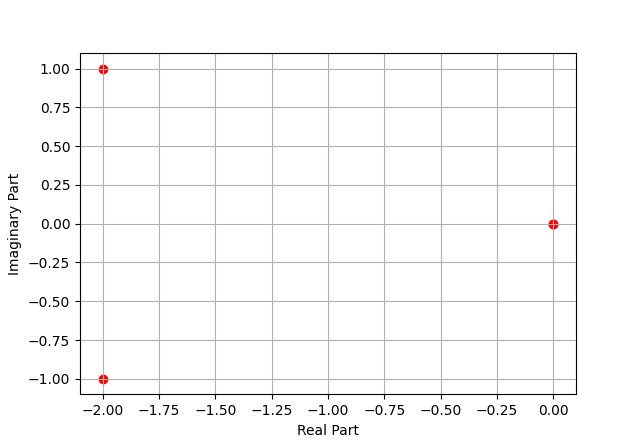
\includegraphics[width=\columnwidth]{graph_1}
\label{figure:ee25-gate4-graph1}
\caption{Location of roots for $k_i=0$,$k_p=-1$}
\end{figure}

\begin{figure}    
    \centering
\graphicspath{ {2021/EC/48/figs} }
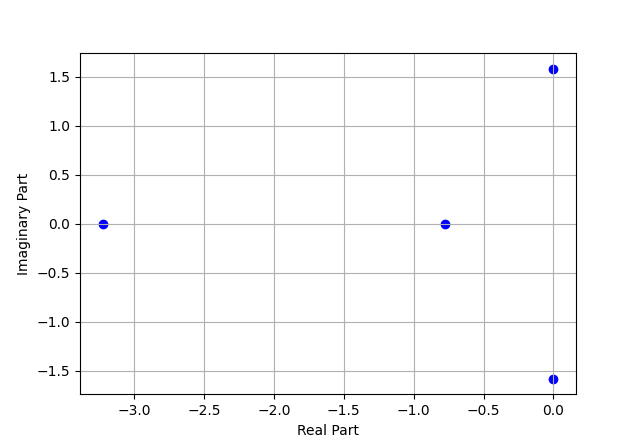
\includegraphics[width=\columnwidth]{graph_2}
\caption{Location of roots for $k_i=0$,$k_p=9$}
\label{figure:ee25-gate4-graph2}
\end{figure}

\begin{figure}    
    \centering
\graphicspath{ {2021/EC/48/figs} }
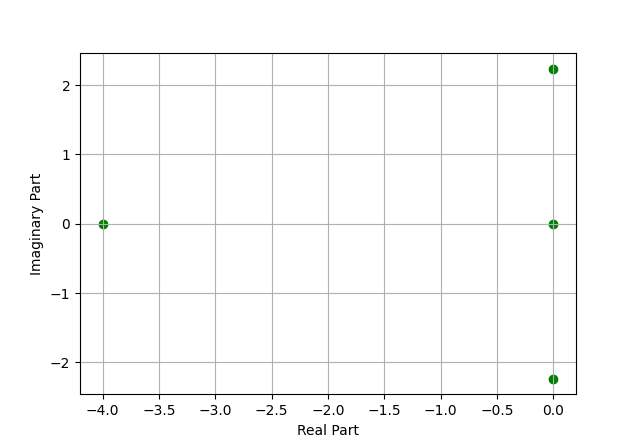
\includegraphics[width=\columnwidth]{graph_3}
\caption{Location of roots for $k_i=3.125$,$k_p=4$}
\label{figure:ee25-gate4-graph3}
\end{figure}

 \item Verification by Nyquist diagrams:\\
 From $\ref{table:ee25-ec48-gate2021}$, if $P=0$ and $-1+0j$ is neither bounded nor unbounded by the contour, then the system is marginally stable.
 For P:
 \begin{align}
     s^4+4s^3+5s^2+2s &= 0\\
     (s+1)^2(s+2) &= 0\\
     \implies P &= 0\\ 
     \implies Z &= N
 \end{align}
 
 
 \begin{figure}[!ht]    
    \centering
\graphicspath{ {2021/EC/48/figs} }
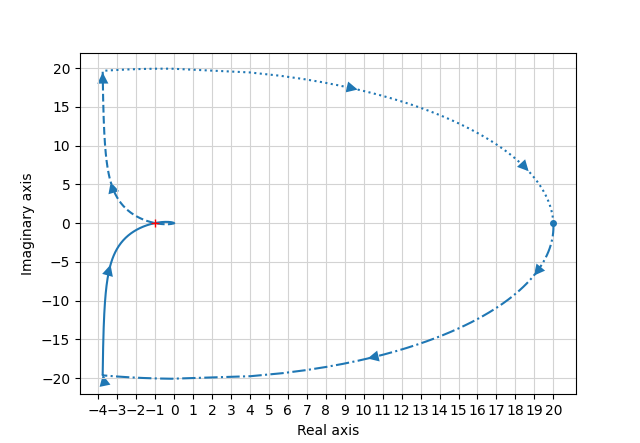
\includegraphics[width=\columnwidth]{plot_1}
\label{figure:ee25-gate4-nyquist1}
\caption{ Nyquist plot for $k_i=0$,$k_p=-1$}
\end{figure}

\begin{figure}[!ht]    
    \centering
\graphicspath{ {2021/EC/48/figs} }
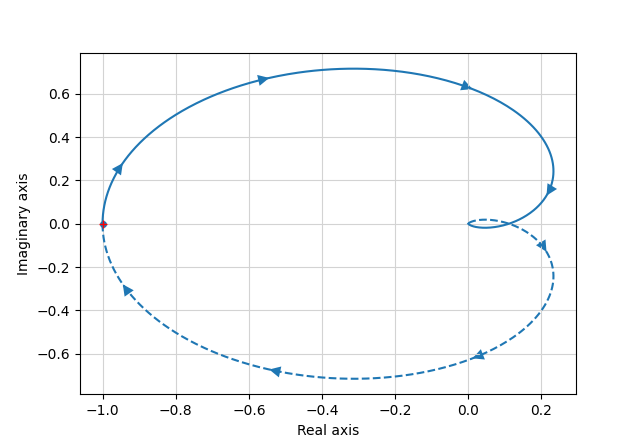
\includegraphics[width=\columnwidth]{plot_2}
\label{figure:ee25-gate4-nyquist2}
\caption{Nyquist plot for $k_i=0$,$k_p=9$}
\end{figure}

\begin{figure}[!ht]    
    \centering
\graphicspath{ {2021/EC/48/figs} }
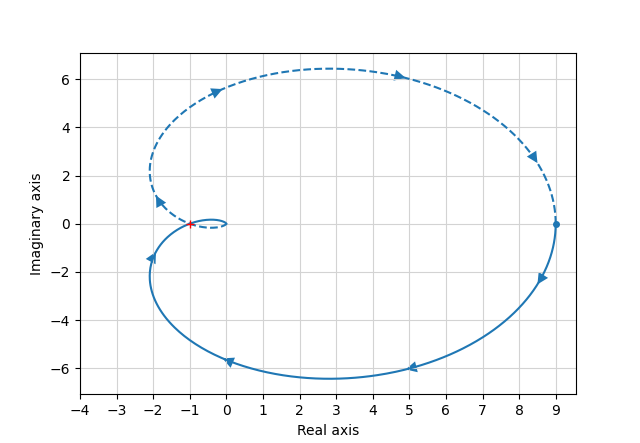
\includegraphics[width=\columnwidth]{plot_3}
\label{figure:ee25-gate4-nyquist3}
\caption{Nyquist plot for for $k_i=3.125$,$k_p=4$}
\end{figure}
     \end{enumerate}

  
   
    



\pagebreak
\item In the given figure, plant $G_p(s)=\frac{2.2}{(1+0.1s)(1+0.4s)(1+1.2s)}$ and compensator $G_c(s)=K\brak{\frac{1+T_1s}{1+T_2s}}$ . The external disturbance input is D(s). It is desired that when the disturbance is a unit step, the steady-state error should not exceed 0.1 unit. The minimum value of K is 
\hfill{(GATE EE 2021)}\\
\begin{figure}[h!]
    \centering
    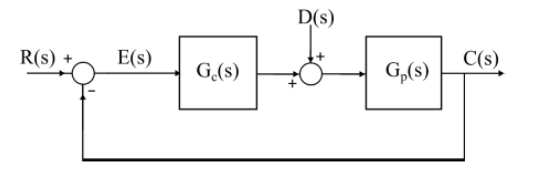
\includegraphics[width=\columnwidth]{2021/EE/47/figs/fig.png}
    \caption{}
    \label{fig:sr40}
\end{figure}
\\
\solution
\iffalse
\documentclass[journal,12pt,twocolumn]{IEEEtran}
\usepackage{cite}
\usepackage{amsmath,amssymb,amsfonts,amsthm}
\usepackage{algorithmic}
\usepackage{graphicx}
\usepackage{textcomp}
\usepackage{xcolor}
\usepackage{txfonts}
\usepackage{listings}
\usepackage{enumitem}
\usepackage{mathtools}
\usepackage{float}
\usepackage{gensymb}
\usepackage{comment}
\usepackage[breaklinks=true]{hyperref}
\usepackage{tkz-euclide} 
\usepackage{listings}
\usepackage{gvv}                                        
\def\inputGnumericTable{}                                 
\usepackage[latin1]{inputenc}                                
\usepackage{color}                                            
\usepackage{array}                                            
\usepackage{longtable}                                       
\usepackage{calc}                                             
\usepackage{multirow}                                         
\usepackage{hhline}                                           
\usepackage{ifthen}                                           
\usepackage{lscape}
\usepackage{amsmath}
\newtheorem{theorem}{Theorem}[section]
\newtheorem{problem}{Problem}
\newtheorem{proposition}{Proposition}[section]
\newtheorem{lemma}{Lemma}[section]
\newtheorem{corollary}[theorem]{Corollary}
\newtheorem{example}{Example}[section]
\newtheorem{definition}[problem]{Definition}
\newcommand{\BEQA}{\begin{eqnarray}}
\newcommand{\EEQA}{\end{eqnarray}}
\newcommand{\define}{\stackrel{\triangle}{=}}
\theoremstyle{remark}
\newtheorem{rem}{Remark}

\usepackage{circuitikz} 

\begin{document}
{\small

\bibliographystyle{IEEEtran}
\vspace{3cm}

\title{GATE 2021 EE 47}
\author{EE23BTECH11045 - Palavelli Srija$^{*}$}

\maketitle

\bigskip

\renewcommand{\thefigure}{\theenumi}
\renewcommand{\thetable}{\theenumi}

\vspace{3cm}
\textbf{Question:} 
In the given figure, plant $G_p(s)=\frac{2.2}{(1+0.1s)(1+0.4s)(1+1.2s)}$ and compensator $G_c(s)=K\brak{\frac{1+T_1s}{1+T_2s}}$ . The external disturbance input is D(s). It is desired that when the disturbance is a unit step, the steady-state error should not exceed 0.1 unit. The minimum value of K is
\begin{figure}[h!]
    \centering
    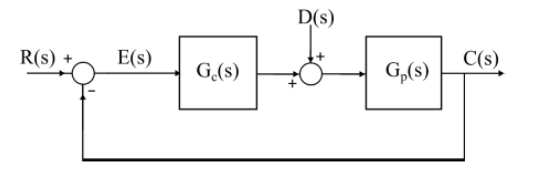
\includegraphics[width=\columnwidth]{2021/EE/47/figs/fig.png}
    \caption{}
    \label{fig:sr40}
\end{figure}
\\
\textbf{Solution:}\\
\fi
\begin{table}[h!]
    \centering
     \begin{tabular}{|c|c|}
        \hline
        \textbf{Symbol}  & \textbf{Value} \\
        \hline
        $G_p(s)$ & $\frac{2.2}{(1+0.1s)(1+0.4s)(1+1.2s)}$\\
         \hline
        $G_c(s)$& $K\brak{\frac{1+T_1s}{1+T_2s}}$  \\
         \hline
        $|e_{ss}|$& $\leq 0.1$\\
         \hline
        $K_{min}$& ??\\
        \hline
    \end{tabular}

    \caption{Input Parameters}
    \label{tab:table_omega}
\end{table}
 
\begin{align}
\text{From \figref{fig:sr40}}\notag\\
E(s) &= R(s)-C(s) \\
\text{Assume R(s)=0}\notag\\
E(s) &= -C(s) \\
C(s) &= \brak{E(s)G_c(s)+D(s)}G_p(s) \\
-E(s) &= \brak{E(s)G_c(s)+D(s)}G_p(s) \\
E(s) &= \frac{-D(s)G_p(s)}{1+G_c(s)G_p(s)} 
\end{align}
Using final value theorem 
\begin{align}
e_{ss} &= \lim_{{t \to \infty}} e(t) = \lim_{{s \to 0}} sE(s)\\
\text{Where}\quad\mathcal{L}\{e(t)\} &= E(s) \notag\\
e_{ss} &= \lim_{{s \to 0}} sE(s) \\
&= \lim_{{s \to 0}} \left(\frac{-sD(s)G_p(s)}{1+G_c(s)G_p(s)} \right) \\
\end{align}
\begin{align}
 D(s)&=\mathcal{L}\{u(t)\}  \notag\\
&=\frac{1}{s}\\
e_{ss} &=\lim_{{s \to 0}} \left(\frac{-s\frac{1}{s}G_p(s)}{1+G_c(s)G_p(s)} \right) \\
&= \lim_{{s \to 0}} \frac{\frac{-2.2}{(1+0.1s)(1+0.4s)(1+1.2s)}}{1+K\left(\frac{1+T_1s}{1+T_2s}\right)\frac{2.2}{(1+0.1s)(1+0.4s)(1+1.2s)}} \\
&= \lim_{{s \to 0}} \frac{-2.2(1+T_2s)}{(1+0.1s)(1+0.4s)(1+1.2s)(1+T_2s)+2.2K(1+T_1s)} \\
|e_{ss}| &= \frac{2.2}{1+2.2K} \\
\text{given}\notag\\ |e_{ss}|&\leq 0.1\\
\frac{2.2}{1+2.2K} &\leq 0.1 \\
K &\geq 9.54 \\
K_{\text{min}} &= 9.54
\end{align}
    %\end{document}

\pagebreak
\item For the closed loop system shown , the transfer function $\frac{E(s)}{R(s)}$ is \\
\begin{figure}[ht]
	\centering
	\includegraphics[width=1\linewidth]{2021/EE/11/figs/questiondia.png}
\end{figure}
\begin{enumerate}[label = (\alph*)]
	\item $\frac{G}{1+GH}$
	\item $\frac{GH}{1+GH}$
	\item $\frac{1}{1+GH}$
	\item $\frac{1}{1+G}$
\end{enumerate} \hfill{(GATE EE 2021)}\\
%\iffalse
\let\negmedspace\undefined
\let\negthickspace\undefined
\documentclass[journal,12pt,twocolumn]{IEEEtran}
\usepackage{cite}
\usepackage{amsmath,amssymb,amsfonts}
\usepackage{graphicx}
\usepackage{textcomp}
\usepackage{xcolor}
\usepackage{txfonts}
\usepackage{listings}
\usepackage{enumitem}
\usepackage{mathtools}
\usepackage{gensymb}
\usepackage{comment}
\usepackage[breaklinks=true]{hyperref}
\usepackage{tkz-euclide} 
\usepackage{listings}
\usepackage{gvv}                                        
\def\inputGnumericTable{}                                 
\usepackage[latin1]{inputenc}                                
\usepackage{color}                                            
\usepackage{array}                                            
\usepackage{longtable}                                       
\usepackage{calc}                                             
\usepackage{multirow}                                         
\usepackage{hhline}                                           
\usepackage{ifthen}                                           
\usepackage{lscape}
\usepackage[export]{adjustbox}
\usepackage{pgfplots}
\newtheorem{theorem}{Theorem}[section]
\newtheorem{problem}{Problem}
\newtheorem{proposition}{Proposition}[section]
\newtheorem{lemma}{Lemma}[section]
\newtheorem{corollary}[theorem]{Corollary}
\newtheorem{example}{Example}[section]
\newtheorem{definition}[problem]{Definition}
\newcommand{\BEQA}{\begin{eqnarray}}
	\newcommand{\EEQA}{\end{eqnarray}}
\newcommand{\define}{\stackrel{\triangle}{=}}
\newtheorem{rem}{Remark}

\begin{document}
	\parindent 0px
	\bibliographystyle{IEEEtran}
	
	\vspace{3cm}
	
	\title{GATE:EE/63}
	\author{EE23BTECH11208 - Manohar K$^{*}$
	}
	\maketitle
	\newpage
	\bigskip
	
	% \renewcommand{\thefigure}{\theenumi}
	% \renewcommand{\thetable}{\theenumi}
	
	
	
\textbf{Question:} For the closed loop system shown , the transfer function $\frac{E(s)}{R(s)}$ is \\
\begin{figure}[ht]
	\centering
	\includegraphics[width=1\linewidth]{figs/questiondia.png}
\end{figure}
\begin{enumerate}[label = (\alph*)]
	\item $\frac{G}{1+GH}$
	\item $\frac{GH}{1+GH}$
	\item $\frac{1}{1+GH}$
	\item $\frac{1}{1+G}$
\end{enumerate} \hfill{(GATE EE 2021)}\\



 \noindent \textbf{Solution:}
	Given,\\
	
	\begin{table}[h]
		\centering
		
\begin{tabular}{|c|c|l|}
\hline
Parameter  & Value & Description   \\             
\hline
$y(0)$     & $0$   & Initial displacement  \\     
 \hline
$y'(0)$    & $0$   & First derivative at $t=0$  \\
 \hline
$y''(0)$   & $0$   & Second derivative at $t=0$ \\
 \hline
$y'''(0)$  & $0$   & Third derivative at $t=0$  \\
 \hline
\end{tabular}


		\caption{Parameters}
		\label{tab:GATE.EE.2021.11}
	\end{table}
	
	\begin{align}
		C(s)&=G \times E(s)\\
		\text{Feedback signal} &= H \times C(s)
	\end{align}
	    
	
	\begin{align}
	      E(s) &= R(s) - H \times C(s)
	\end{align}
	from eq (1),     
	\begin{align}
		E(s) &= R(s) - H \times G \times E(s)
	\end{align}
	\begin{align}
		E(s) +  H \times G \times E(s) &= R(s)
		\end{align}
		\begin{align}
					\therefore \frac{E(s)}{R(s)} &= \frac{1}{1 + GH}
	\end{align} 
	
	
	
	
\end{document}

\pagebreak

Consider two 16-point sequences x\sbrak{n} and h\sbrak{n}. Let the linear convolution of x\sbrak{n} and h\sbrak{n} be denoted by y\sbrak{n}, while z\sbrak{n} denotes the 16-point inverse discrete Fourier transform \brak{IDFT} of the product of the 16-point DFTs of x\brak{n} and h\sbrak{n}. The values of k for which z\sbrak{k} = y\sbrak{k} are 
\begin{enumerate}
    \item $k = 0, 1, 2, 3, ... , 15$
    \item $k = 0$
    \item $k = 15$
    \item $k = 0$ and $k = 15$
\end{enumerate}
\hfill(GATE EC 2021)\\
\solution
\iffalse
\let\negmedspace\undefined
\let\negthickspace\undefined
\documentclass[journal,12pt,twocolumn]{IEEEtran}
\usepackage{cite}
\usepackage{amsmath,amssymb,amsfonts,amsthm}
\usepackage{algorithmic}
\usepackage{graphicx}
\usepackage{textcomp}
\usepackage{xcolor}
\usepackage{txfonts}
\usepackage{listings}
\usepackage{enumitem}
\usepackage{mathtools}
\usepackage{gensymb}
\usepackage{comment}
\usepackage[breaklinks=true]{hyperref}
\usepackage{tkz-euclide} 
\usepackage{listings}
\usepackage{gvv}                                        
\def\inputGnumericTable{}                                 
\usepackage[latin1]{inputenc}                                
\usepackage{color}                                            
\usepackage{array}                                            
\usepackage{longtable}                                       
\usepackage{calc}                                             
\usepackage{multirow}                                         
\usepackage{hhline}                                           
\usepackage{ifthen}                                           
\usepackage{lscape}
\usepackage{placeins}
\usepackage{xparse}


\newtheorem{theorem}{Theorem}[section]
\newtheorem{problem}{Problem}
\newtheorem{proposition}{Proposition}[section]
\newtheorem{lemma}{Lemma}[section]
\newtheorem{corollary}[theorem]{Corollary}
\newtheorem{example}{Example}[section]
\newtheorem{definition}[problem]{Definition}
\newcommand{\BEQA}{\begin{eqnarray}}
\newcommand{\EEQA}{\end{eqnarray}}
\newcommand{\define}{\stackrel{\triangle}{=}}
\theoremstyle{remark}
\newtheorem{rem}{Remark}

\graphicspath{ {./figs/} } 

\begin{document}

\bibliographystyle{IEEEtran}
\vspace{3cm}

\Large\title{GATE 2021 EC 5}
\large\author{EE23BTECH11032 - Kaustubh Parag Khachane $^{*}$% <-this % stops a space
}
\maketitle
\newpage
\bigskip

\renewcommand{\thefigure}{\theenumi}
\renewcommand{\thetable}{\theenumi}
\large\textbf{Question GATE 21 EC 5} :\\
Consider two 16-point sequences x\sbrak{n} and h\sbrak{n}. Let the linear convolution of x\sbrak{n} and h\sbrak{n} be denoted by y\sbrak{n}, while z\sbrak{n} denotes the 16-point inverse discrete Fourier transform \brak{IDFT} of the product of the 16-point DFTs of x\brak{n} and h\sbrak{n}. The values of k for which z\sbrak{k} = y\sbrak{k} are 
\begin{enumerate}
    \item $k = 0, 1, 2, 3, ... , 15$
    \item $k = 0$
    \item $k = 15$
    \item $k = 0$ and $k = 15$
\end{enumerate}
\hfill(GATE EC 2021)\\
\solution\\
\fi
\begin{table}[!ht] 
\centering
\setlength{\extrarowheight}{8pt}
\begin{tabular}{|l|l|}
    \hline
    \textbf{Parameter} & \textbf{Description}  \\\hline
     x\sbrak{n} & Given 16 point sequence \\\hline
     h\sbrak{n} &  Given 16 point sequence \\\hline
     y\sbrak{n} & Linear convolution of x\sbrak{n} and h\sbrak{n} \\\hline
     z\sbrak{n} & IDFT of products of DFTs of h\sbrak{n} and x\sbrak{n} \\\hline
     N & number of terms \brak{16} \\\hline
    \end{tabular}
  \vspace{4mm}
 \caption{Parameter Table}
 \label{tab:table0_ec5}
\end{table}

We can write z\sbrak{n} as ,
\begin{align}
    z\sbrak{n} = IDFT\sbrak{X\sbrak{f}H\sbrak{f}}
\end{align}
We know that product in frequency domain is convolution in time domain. However, z\sbrak{n} is not linear convolution of x\sbrak{n} and h\sbrak{n} in the time domain due to periodicity of DFT. Point-wise multiplication in the frequency domain (product of DFTs) doesn't translate directly to convolution in the time domain due to periodicity and potential aliasing.\\
z\sbrak{n} is the circular convolution of x\sbrak{n} and h\sbrak{n}. Using the formula for circular convolution,
\begin{align}
    z\sbrak{n} = \sum_{m = -\infty}^{\infty}\brak{h\sbrak{m} \sum_{p = -\infty}^{\infty}x\sbrak{n - m -pN}} \label{eq:eq1_g21ec5}
\end{align}
y\sbrak{n} is a linear convolution of x\sbrak{n} and h\sbrak{n}.
\begin{align}
    y\sbrak{n} = \sum_{m = -\infty}^{\infty} x\brak{m} h\sbrak{n-m}
\end{align}
Each term of y\sbrak{n} will be sum of products of terms of x\sbrak{n} and h\sbrak{n}. The number of terms in each summation will go from 1 for $n=1$ to 16 for $n=15$. \\
z\sbrak{n} is expressed as sum of 15 terms for all permissible values of n using $p=0$ or $p=1$ in \eqref{eq:eq1_g21ec5}.
\\ Thus,$z\sbrak{k} = y\sbrak{k}$ can be possible for only $k=15$.
\\ For $k = 15$,
\begin{align}
    y\sbrak{15} &= x\sbrak{0}h\sbrak{15} +  x\sbrak{1}h\sbrak{14} + ...  x\sbrak{15}h\sbrak{0} 
\end{align}
Using p = 0  in \eqref{eq:eq1_g21ec5},
\begin{align}
    z\sbrak{15} &= h\sbrak{0} x\sbrak{15} + h\sbrak{1} x\sbrak{14} + ... h\sbrak{15} x\sbrak{0}\\
    &=  x\sbrak{0}h\sbrak{15} +  x\sbrak{1}h\sbrak{14} + ...  x\sbrak{15}h\sbrak{0} 
\end{align}
Thus , z\sbrak{15} = y\sbrak{15}.\\
Graphically, let 
\begin{align}
    x &= \sbrak{1,2,3,4,....,16}\\
    h &= \sbrak{1,1,1,1, ... 1}
\end{align}
Then the plot for z and y is as shown bellow.
\begin{figure}[!ht]
\centering
\begin{center}
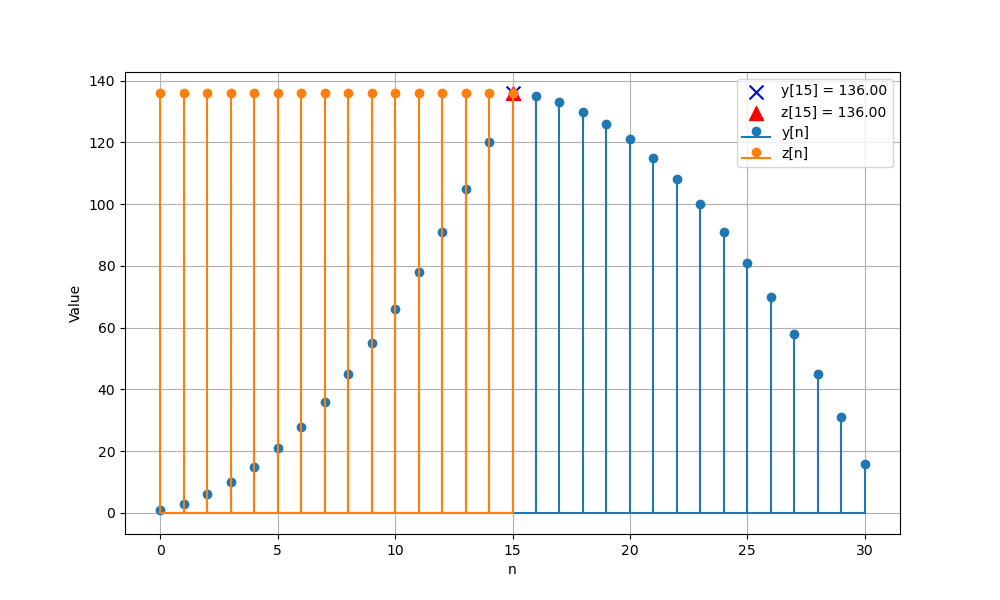
\includegraphics[width=\columnwidth]{2021/EC/5/figs/Figure_1.png}
\end{center}
\caption{Plot of y\sbrak{n} and z\sbrak{n}}
\end{figure}

\pagebreak
\item The input signal shown below \\
\input{2021/IN/44/figs/xn}\\
is passed through the filter with following taps\\
\input{2021/IN/44/figs/n}\\
The number of non-zero output samples is \underline{\hspace{1cm}}.\\
\hfill(GATE IN 2021)
\solution
\iffalse
\let\negmedspace\undefined
\let\negthickspace\undefined
\documentclass[journal,12pt,twocolumn]{IEEEtran}
\usepackage{cite}
\usepackage{amsmath,amssymb,amsfonts,amsthm}
\usepackage{algorithmic}
\usepackage{graphicx}
\usepackage{textcomp}
\usepackage{xcolor}
\usepackage{txfonts}
\usepackage{listings}
\usepackage{enumitem}
\usepackage{mathtools}
\usepackage{gensymb}
\usepackage{comment}
\usepackage[breaklinks=true]{hyperref}
\usepackage{tkz-euclide} 
\usepackage{listings}
\usepackage{gvv}
\def\inputGnumericTable{}                                 
\usepackage[latin1]{inputenc}                                
\usepackage{color}                                            
\usepackage{array}                                            
\usepackage{longtable}                                       
\usepackage{calc}                                             
\usepackage{multirow}                                         
\usepackage{hhline}                                           
\usepackage{ifthen}                                           
\usepackage{lscape}

\newtheorem{theorem}{Theorem}[section]
\newtheorem{problem}{Problem}
\newtheorem{proposition}{Proposition}[section]
\newtheorem{lemma}{Lemma}[section]
\newtheorem{corollary}[theorem]{Corollary}
\newtheorem{example}{Example}[section]
\newtheorem{definition}[problem]{Definition}
\newcommand{\BEQA}{\begin{eqnarray}}
\newcommand{\EEQA}{\end{eqnarray}}
\newcommand{\define}{\stackrel{\triangle}{=}}
\theoremstyle{remark}
\newtheorem{rem}{Remark}

\begin{document}

\bibliographystyle{IEEEtran}
\vspace{3cm}

\title{GATE IN21 44}
\author{EE23BTECH11043 - BHUVANESH SUNIL NEHETE$^{*}$% <-this % stops a space
}
\maketitle
\newpage
\bigskip

\renewcommand{\thefigure}{\theenumi}
\renewcommand{\thetable}{\theenumi}

\bibliographystyle{IEEEtran}

\textbf{Question:}
The input signal shown below \\
\input{2021/IN/44/figs/xn}\\
is passed through the filter with following taps\\
\input{2021/IN/44/figs/n}\\
The number of non-zero output samples is \underline{\hspace{1cm}}.\\

\solution
\fi
\begin{align}
    h\sbrak{n}=-\delta\sbrak{n}+2\delta\sbrak{n+1}-\delta\sbrak{n+2}
\end{align}
\begin{align}
    y\sbrak{n}&=x\sbrak{n}*h\sbrak{n}\\
    &=x\sbrak{n}*\brak{-\delta\sbrak{n}+2\delta\sbrak{n+1}-\delta\sbrak{n+2}}\\
    y\sbrak{n}&=-x\sbrak{n}+2x\sbrak{n+1}-x\sbrak{n+2}
\end{align}

\input{2021/IN/44/figs/yn}
The number of non-zero output samples is $10$.

\begin{figure}
    \centering
    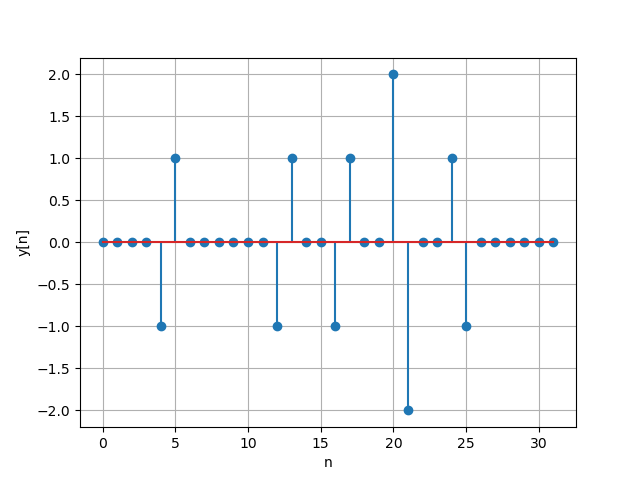
\includegraphics[width=1\linewidth]{2021/IN/44/figs/fig.png}
\end{figure}

\pagebreak
\end{enumerate}
